% data_ex.tex
\documentclass[main.tex]{subfiles}
\begin{document}
\chapter{Trends in Print Force and Extrusion Speed} \label{ch:data_ex}
\section{Foreword} \label{sec:fw_dataex}

Material Extrusion (ME), also known as Fused Filament Fabrication (FFF), is the most prevalent Additive Manufacturing (AM) technology due to the broad range of materials and equipment available, generally attainable at a fraction of the cost of other AM processes. While ME has gradually found niche applications outside of the casual user, including implementations in the automotive and aerospace sectors, the slow print speed of the process represents a major pain point of the technology that limits the scope of its adoption. Additionally, process control relies mostly on temperature readings, and there is room for improvement in terms of variations in volumetric throughput and process fluctuations. For this reason, this study uses a customized ME machine with a built-in force sensor and encoder that allows real time acquisition of force and filament print speed data, generating knowledge aimed at maximizing the print speed of ME and improving the understanding of the underlying process physics that can lead to improved print quality and consistency. 

In the context of this dissertation, every ML solution begins with a data acquisition and exploration step. This study represents just that, as it allowed the researcher to understand an FFF machine with sensors, develop data filtering techniques, and the deployment of automation protocols that made acquisition of the training and validation data sets of the ML model a lot easier and faster. Finally, and as an added bonus, the results of this study shed some light into the current limitations intrinsic to two of the most widely used melting models for FFF: the Bellini \emph{et al.} model, and the Osswald, Puentes, Kattinger model, as both require measurements of filament force and speed to compare data with theoretical predictions \textemdash a feat that was uncommon at the time of this body of work.

\section{Equipment and Materials} \label{ssec:mat_data}

\subsection{Printer Setup} \label{ssec:printer}

For this study, an ME 3D printer (Minilab by FusedForm, Colombia) using a 0.4 mm nozzle and capable of printing 1.75 mm filament was equipped with a customized force sensor and thermistor built into the printhead, as well as an encoder that records the extruded filament length over time. The concentric force sensor was positioned just above the hot end, in a Bowden extruder architecture. These modifications permit recording and visualization of live force, filament speed, and temperature data collected during the printing process, while maintaining the original performance and functionality of the 3D printer. The generated data was collected using an Arduino board sampling at a frequency of 5 Hz, connected to MATLAB for visualization, processing, and logging. The printhead setup and encoder positioning can be seen in detail in Figure \ref{fig:printsetup}. This setup has the added benefit of allowing detection of filament slippage, if present. As shown in Figure \ref{fig:printsetup} the external ring of the force sensor sits on the extruder carrier base, secured by the extruder carrier lid. The modified hot-end sits on the internal ring of the force sensor, secured in place by the hot-end-sensor coupler. A small clearance between the carrier lid and the sensor permits the filament force to be transmitted through the assembly and detected by the DAQ system.

\begin{figure}[!htbp]
	\center
	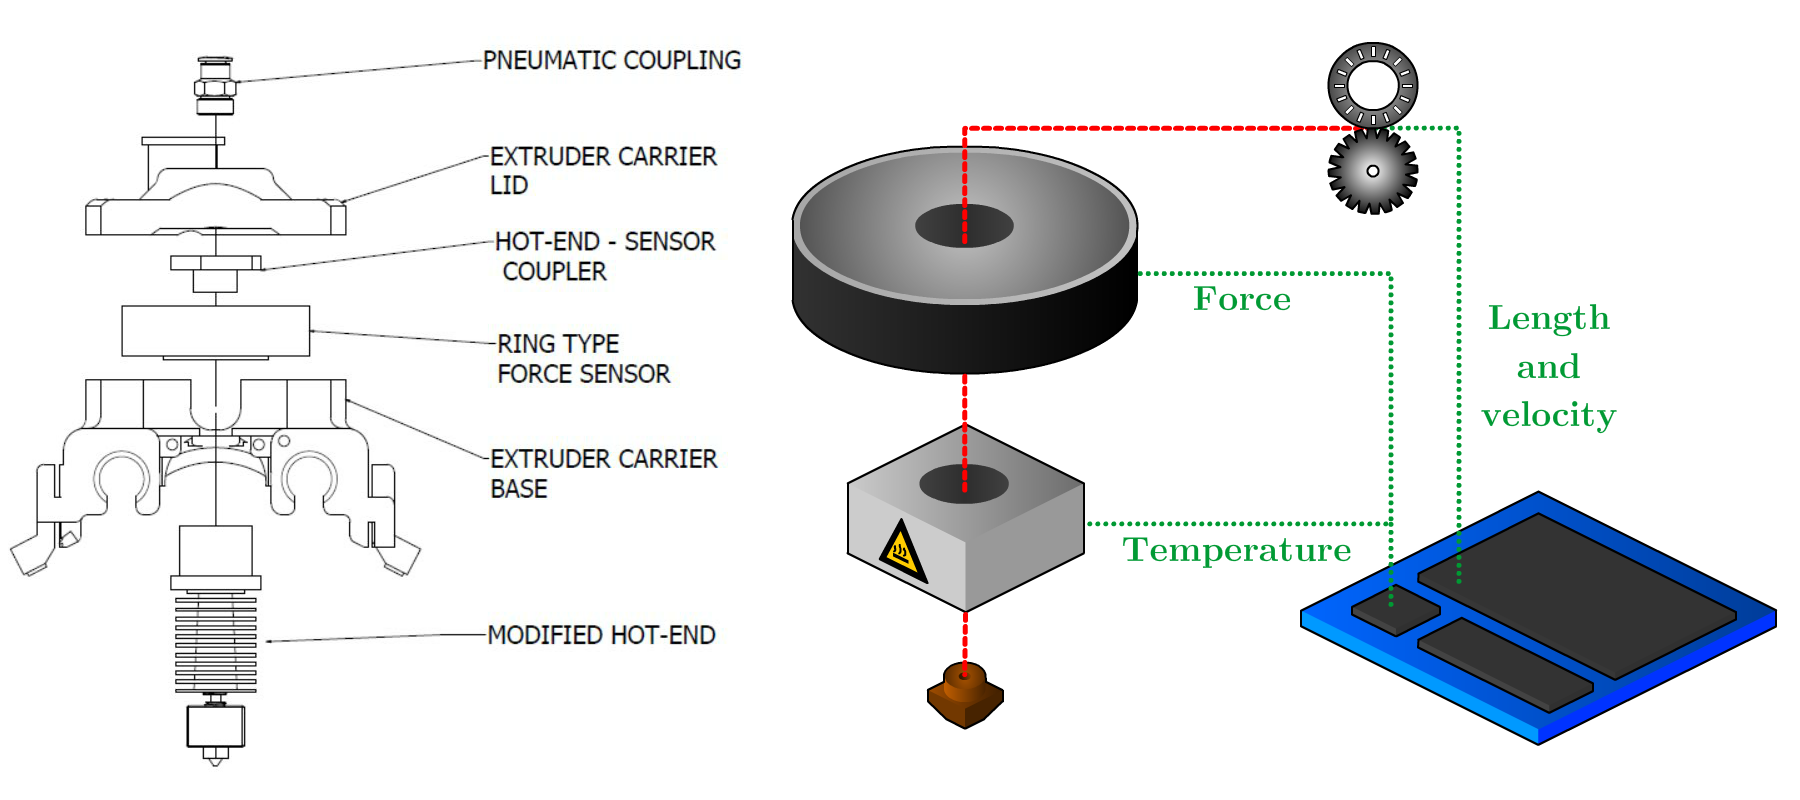
\includegraphics[width=0.9\linewidth, keepaspectratio]{Forcesetup}
	\caption{Assembly shown on the left. Schematic of sensor placement on the right.} \label{fig:printsetup}
\end{figure}

\subsection{Materials} \label{ssec:materials_dataex}

Two materials were chosen to perform the experiments pertaining to this body of work: a customized ABS filament, extruded in-house, and a commercially available PLA filament, each with a nominal diameter of 1.75 mm. The ABS filament was produced using the SABIC Cycolac™ MG94 material. This is an ABS resin traditionally used for injection molding thin-walled parts, as well as ME filament. With a reported Melt Flow Index of 11.7 g/10 min, it is an ideal resin for both the ME and extrusion processes \cite{sabic2016}. The extrusion setup consisted of a single screw extruder (Extrudex EDN 45X30D, Germany) with 45 mm screw diameter and L/D ratio of 30D. The hot melt was extruded at 205 ºC through a circular die with a 4.2 mm diameter. It was then guided through a pre-skinner into a vacuum-assisted, heated water bath (Conair, USA) to cool the extrudate whilst minimizing void formation. The solidified filament then passes through a 3-axis laser micrometer (LaserLinc, USA) and a belt puller (Conair, USA) in a control loop that allows adjustment of the pull speed to keep the extrudate within specification. The desired filament dimensions were a diameter of 1.75 mm with a tolerance of ±0.02 mm. A schematic of the extrusion setup can be seen in Figure \ref{fig:ex_line}. The PLA filament used was the commercially available "Natural PLA PRO" filament sold by Matterhackers, chosen to minimize the effect of colorants/additives to the composition of the filament. Steps were taken to ensure that all the acquired spools of material came from the same lot as to guarantee that processing conditions during the extrusion process were constant. Figure \ref{fig:rheo} shows the complex viscosity for each material, as measured using a 25 mm parallel plate rheometer and a 1 mm gap \cite{ColonQuintana2020}.

\begin{figure}[!htbp]
	\center
	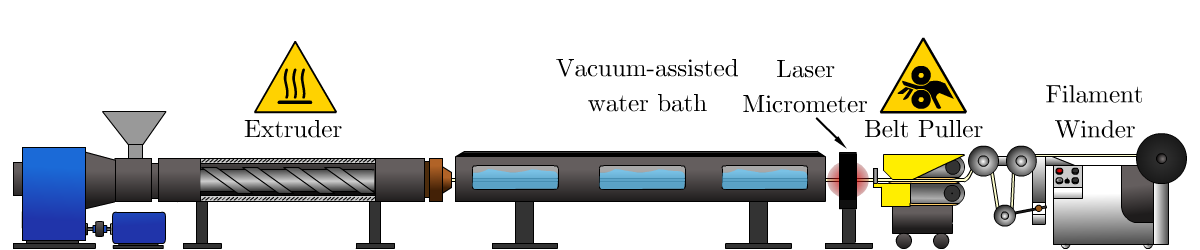
\includegraphics[width=0.9\linewidth, keepaspectratio]{Extrusion_line}
	\caption{Extrusion line used to produce ABS filament} \label{fig:ex_line}
\end{figure}

\begin{figure}[!htbp]
	\center
	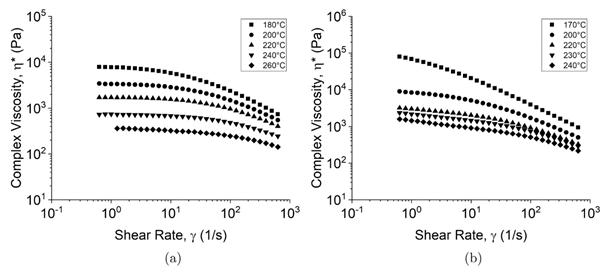
\includegraphics[width=\linewidth, keepaspectratio]{rheology}
	\caption{Shear rate dependency for a) PLA and b) ABS} \label{fig:rheo}
\end{figure}

\section{Design of Experiments} \label{sec:doe_data_ex}

A set of preliminary prints were designed with the goal of exploring the raw data, post processing requirements, and detection of lurking variables. In these experiments, the effect of temperature and print speed upon stable printing conditions in terms of required filament force was observed through the execution of several cylindrical toolpath files, where the printhead movement velocity was changed from 15 mm/s in increments of 5 mm/s every 15 layers, each with a thickness of 0.35 mm. To minimize the effects of varying accelerations during the test, a cylindrical geometry with a radius of 75 mm, printed in continuous helical mode was chosen as the benchmark part, as schematized in Figure \ref{fig:cyl_shak}. This ensures that changes in filament force and velocity stem mostly from the extrusion process and not due to toolpath considerations. To verify the effect of print temperature upon the required extrusion force, each material was printed at three different temperatures: 200, 215 and 230°C for PLA, and 215, 230 and 245°C for ABS. Close attention was paid to variability between prints performed at the same print conditions, as well as the maximum stable print speed for each material-temperature pairing.

\begin{figure}[!htbp]
	\center
	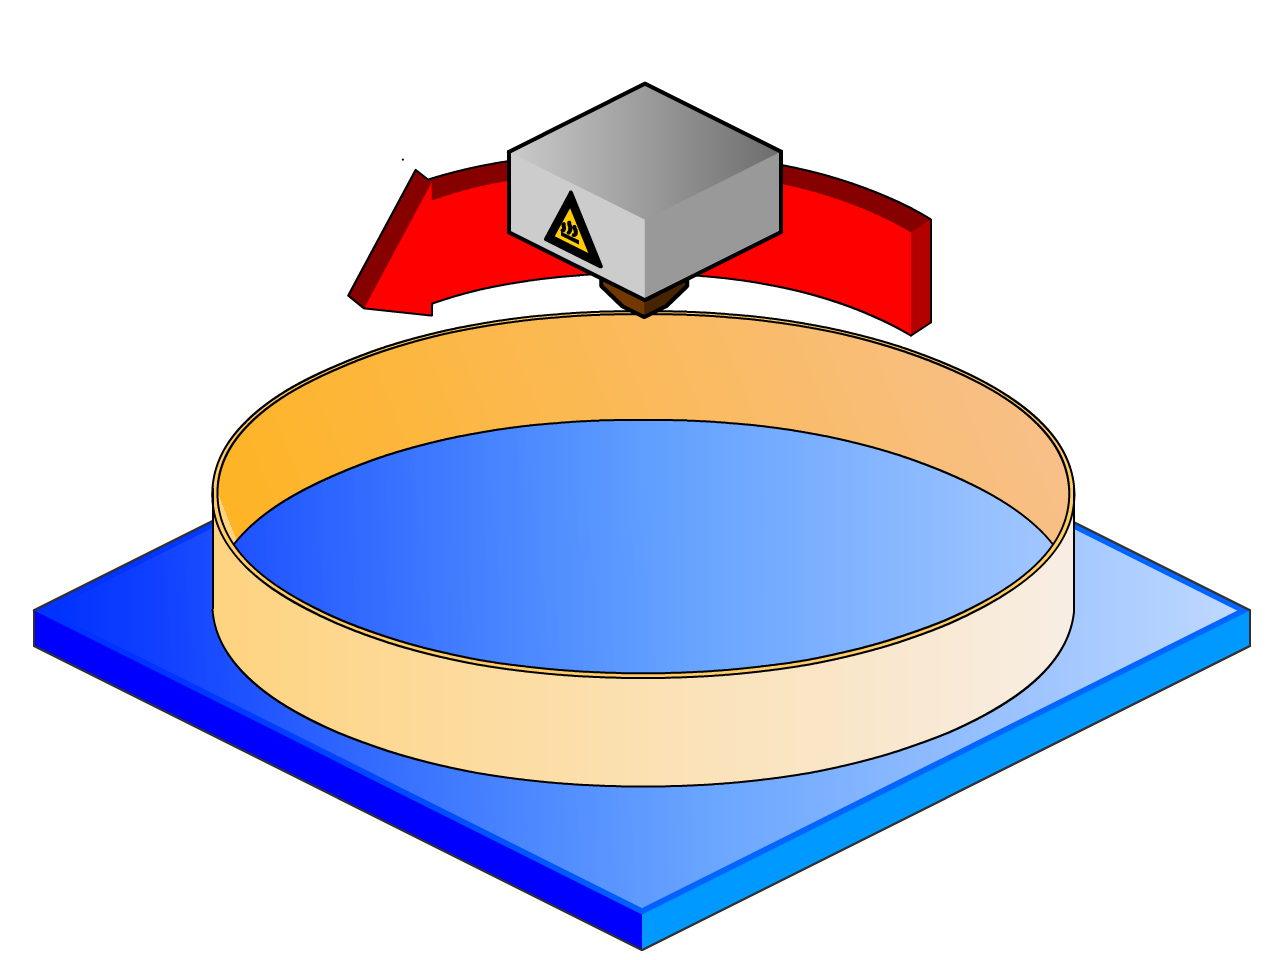
\includegraphics[width=0.6\linewidth, keepaspectratio]{cyl_shakira}
	\caption{Helical cylinder experiment} \label{fig:cyl_shak}
\end{figure}

Once conclusions were drawn from the preliminary set of experiments, the same geometry would be reprinted using a toolpath file that guarantees a comparable number of data points to be collected for each print speed-print temperature-material pairing, as well as utilizing optimal printing conditions and data acquisition considerations. 

\section{Results}\label{sec:res_data_ex}
\subsection{Considerations Derived from Preliminary Tests}

Preliminary tests show that the physical limitation of the setup lies between 20 and 25 N of force acting upon the filament. At this level of force, slippage occurs in the drive wheel mechanism that drives the material towards the nozzle, causing the mass throughput to become discontinuous. This behavior manifested itself on the data as a sudden drop in the measured filament force and was accompanied by an audible click on the driving wheel. Each material-temperature pairing reached this threshold at different print speeds. Once this phenomenon was observed in a recurring manner, data acquisition was stopped to minimize the number of outliers and noise.
 
The characteristics of the ME printing process can be best described using a 2D plot, calculating the filament speed against the force within the nozzle. Filament speed is derived from the length data of extruded filament recorded by an encoder, and should not be confused with the printhead movement speed, which is followed by the machine after interpreting gcode.
 
Figure \ref{fig:unp_data} shows the unprocessed signals of length (bottom), the derived speed (middle) and resulting force (top) of a representative test print, made using PLA printed at 230°C. When looking at the plots of unprocessed signals, noise can be observed in the datasets of force and filament speed. Therefore, a combination of visualization and simple signal processing techniques are required to improve the signal to noise ratio of the datasets.

\begin{figure}[!htbp]
	\center
	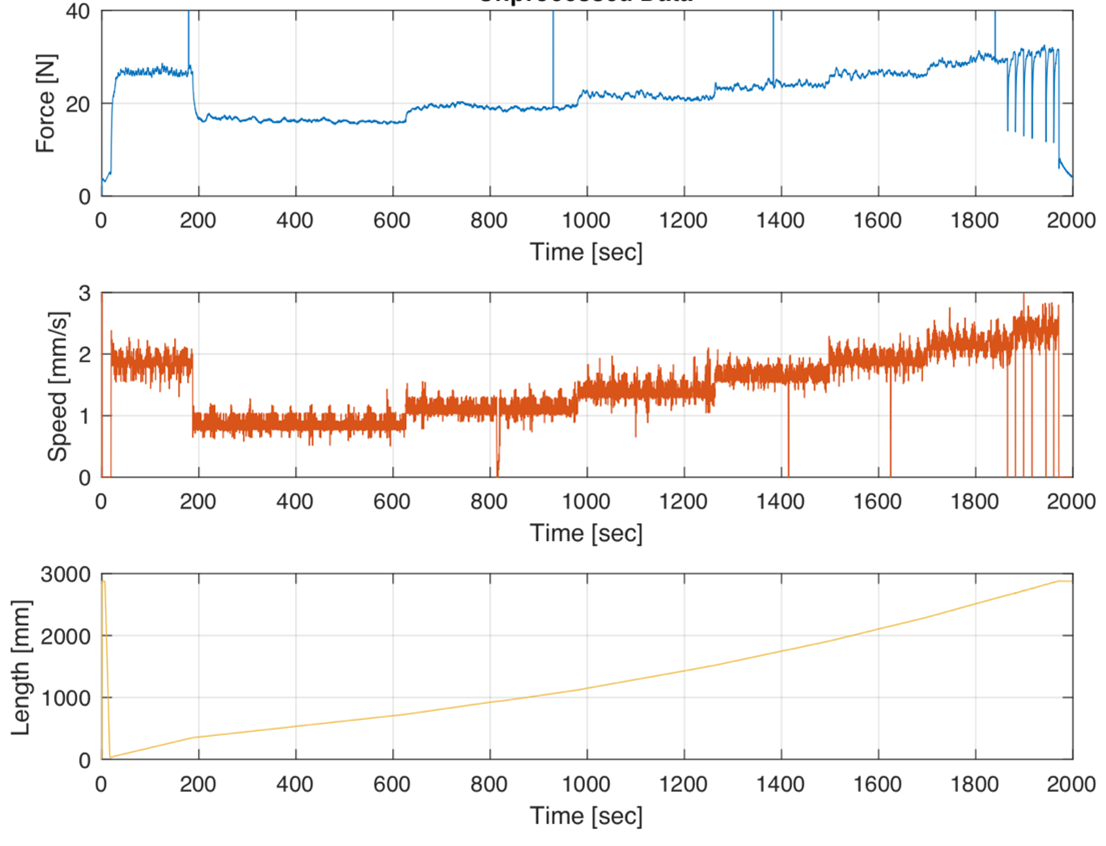
\includegraphics[width=\linewidth, keepaspectratio]{unp_signal}
	\caption{Raw signal data length (bottom), derived speed (middle), and force (top).} \label{fig:unp_data}
\end{figure}

In this example, the first 200 seconds of data are eliminated, as these constitute the time necessary to add the brim to the print, which is necessary to stabilize the cylinder. Datapoints above 1800 seconds are removed as well due to slippage of the filament and high variability within the signal. To remove the amplified noise of the derived speed signal, a moving average filter, applied to the length data showed the best results while keeping most of the signal information. Different parameters for the sliding window of length $k$ across neighboring elements of the length signal have been tested and number of 20 has been found most effective for this application, using a total of 7100 points in the dataset. Deriving the processed length data using the moving average with a sliding window $k$ of 20 shows good results on the filament speed signal in comparison with the unprocessed speed signal. This is better illustrated in Figure \ref{fig:pandu_1}. The oscillating nature of the post processed signal is of unknown origin, but could be related to either the duty cycle of the heater, or small variations in the filament tension that occurred as the toolpath reproduced the circular geometry of the helix. Figure \ref{fig:pandu_2} shows the comparison of processed and unprocessed force vs. filament speed data, where the reduction of noise is apparent.

\begin{figure}[!htbp]
	\center
	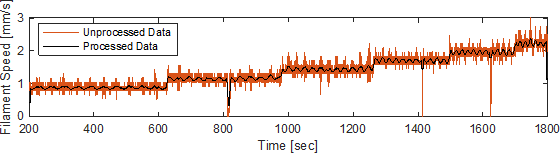
\includegraphics[width=\linewidth, keepaspectratio]{pandu}
	\caption{Comparison of processed and unprocessed filament speed data.} \label{fig:pandu_1}
\end{figure}

\begin{figure}[!htbp]
	\center
	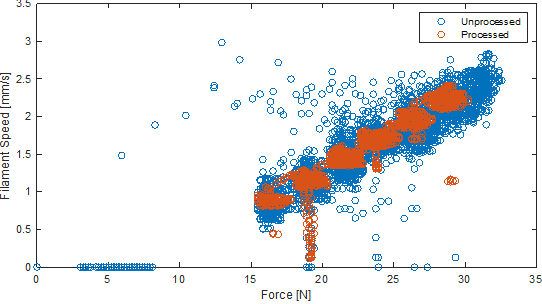
\includegraphics[width=\linewidth, keepaspectratio]{pandu_2}
	\caption{Comparison of processed and unprocessed filament speed vs. force within the nozzle of an FFF printer. PLA printed at 230°C.} \label{fig:pandu_2}
\end{figure}

\pagebreak

Analysis of the post-processed data yielded the following general observations:
\begin{enumerate}
	\item Increasing the hot end temperature allowed the printer to achieve higher filament velocities at lower forces.
	\item Printing at 215°C proved to be unreliable and hard to reproduce, even at lower printing speeds.
	\item Repeatability of results proved to be challenging. Potential causes were determined to be humidity absorbed by the material due to environmental exposure to moisture, partial clog of the nozzle after prolonged use, and additional filament tension caused by the weight of the filament spool preventing an unwinding motion of the material. 
\end{enumerate}

From the conclusions drawn from the preliminary results, the following adjustments were made to the experiment:

\begin{enumerate}
	\item Filament segments were unspooled prior to any experiment to prevent noise originating from filament tension prior to a spool revolution mid-print.
	\item A nozzle cleaning protocol was established, where the printhead would be disassembled, cleaned, and the brass nozzle would be burned at 500°C for 30 minutes to prevent problems arising from nozzle clogging or material degradation. This procedure was executed every time there was a switch in the print material, or every 10 prints, whichever occurred first.
	\item The materials would be dried for a minimum of 3 hours prior to the start of any experiment. This is to minimize the influence of absorbed humidity upon the final materials. ABS was dried at 80°C and PLA at 50°C.
	\item The toolpath file was modified to ensure that each printhead movement speed possessed the same approximate data collection time, as opposed to the same number of print layers. The selected number of layers per printhead movement speed can be seen in Table \ref{tab:layer_time}.
\end{enumerate}

\begin{table}[!htbp] 
	\renewcommand{\arraystretch}{1.5}
	\centering
	\caption{Number of layers per print head movement speed.}
	\newcolumntype{C}{ >{\centering\arraybackslash} m{0.25\linewidth} }
	\newcolumntype{M}{ >{\centering\arraybackslash} m{0.15\linewidth} }
	\begin{tabular}{C C M M} 
		\toprule
		\textbf{Movement speed $[mm/min]$} & \textbf{Movement speed $[mm/s]$} & 
		 \textbf{Time per layer $[s]$} & \textbf{Number of layers}\\
		\midrule
		900 & 15 & 31.41 & 8\\
		1200 & 20 & 23.56 & 10\\
		1500 & 25 & 18.85 & 13\\
		1800 & 30 & 15.71 & 15\\
		2100 & 35 & 13.46 & 18\\
		2400 & 40 & 11.78 & 20\\
		2700 & 45 & 10.47 & 23\\
		3100 & 50 & 9.42 & 25\\
		\bottomrule
	\end{tabular}
	\label{tab:layer_time}
\end{table}

\subsection{Results from Modified Tests}
Results obtained using the modified printing protocol yielded mostly reproducible data. Starting with the ABS material, 5 separate replications of the experiment produced Filament Speed versus Force plots that aligned well with each other. Figure \ref{fig:ABS_230} displays the collected data on the same plot with a transparency filter. Solid areas indicate a denser data cloud. The general trend appears to show an inflection point around the $2 mm/s$ speed mark.

\begin{figure}[!htbp]
	\center
	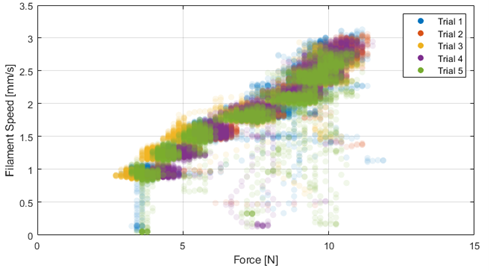
\includegraphics[width=\linewidth, keepaspectratio]{ABS230}
	\caption{Alpha plot for 5 trials of ABS printed at 230°C.} \label{fig:ABS_230}
\end{figure}

The same experiment performed using 245°C as the printing temperature produced similar results, although with a larger data spread. The general trend confirms what is intuitive: higher printing temperatures allows the machine to reach higher extrusion velocities at lower force requirements. The cause of the spread of the data is not fully understood: monitoring the average printing temperature for each trial showed variability of up to 6°C between replicates. It is unknown if the variations between each print replication are caused exclusively by the temperature variations. Variability in the average printing temperature between replicates was most likely caused by approaching the printer’s upper printing temperature limit, causing the setup difficulty at sustaining the 245°C set value. These results are summarized in Figure \ref{fig:ABS_245}. Note how once again, around the $2 mm/s$ mark there appears to be a change in the trend of the data. Table \ref{tab:data_ex_temp} displays the recorded average temperature for each trial. 

\begin{figure}[!htbp]
	\center
	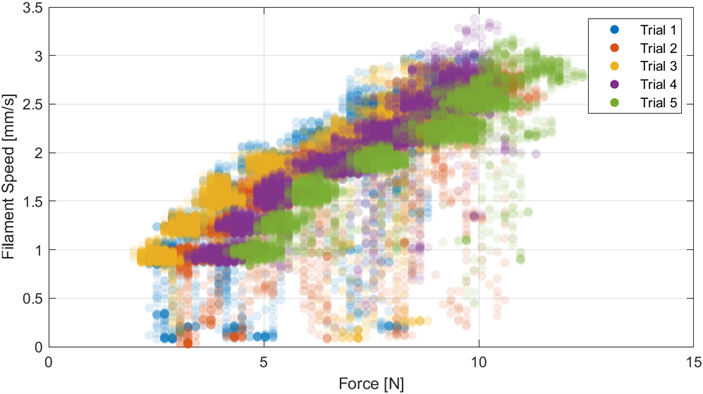
\includegraphics[width=\linewidth, keepaspectratio]{ABS245}
	\caption{Alpha plot for 5 trials of ABS printed at 245°C.} \label{fig:ABS_245}
\end{figure}

\begin{table}[!htbp] 
	\renewcommand{\arraystretch}{1.5}
	\centering
	\caption{Average print temperature for ABS 245°C trials.}
	\newcolumntype{C}{ >{\centering\arraybackslash} m{0.25\linewidth} }
	\newcolumntype{M}{ >{\centering\arraybackslash} m{0.15\linewidth} }
	\begin{tabular}{M C} 
		\toprule
		\textbf{Trial} & \textbf{Average Print Temperature $[^\circ C]$}\\
		\midrule
		1 & 241.38\\
		2 & 231.81\\
		3 & 241.23\\
		4 & 251.60\\
		5 & 241.21\\
		\bottomrule
	\end{tabular}
	\label{tab:data_ex_temp}
\end{table}

For the PLA material, the most notable difference in behavior with respect to the ABS plots was observed in the general trend of the data clusters. For PLA printed at 230°C, an inflection point in the behavior of the data was not observed. This is illustrated in Figure \ref{fig:PLA_230}. Additionally, the data clusters did not overlap as consistently as with ABS. It is unknown if this difference stems from material properties, or other factors not taken into consideration for this study, such as fluctuations in the filament diameter.

\begin{figure}[!htbp]
	\center
	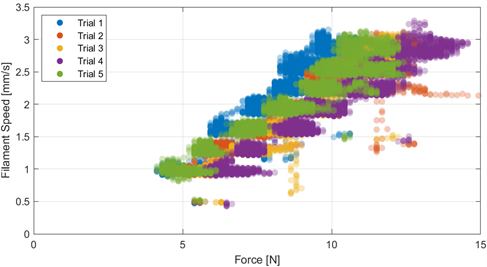
\includegraphics[width=\linewidth, keepaspectratio]{PLA230}
	\caption{Alpha plot for 5 trials of PLA printed at 230°C.} \label{fig:PLA_230}
\end{figure}

Comparing both materials shows that the PLA based material generally requires higher forces to achieve comparable filament velocities to its ABS counterpart. This can be seen in Figure \ref{fig:compPLAABS}, where a characteristic cluster of data was selected for each material and plotted on the same graph for comparative purposes. This result is particularly interesting, given that in general the complex viscosity of ABS tends to be either higher or similar to that of PLA when compared at a fixed shear rate and temperature, as can be seen in Figure \ref{fig:rheo}.


\begin{figure}[!htbp]
	\center
	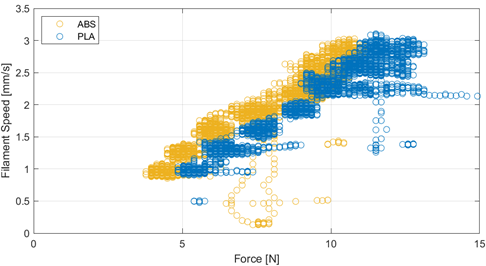
\includegraphics[width=\linewidth, keepaspectratio]{compABSPLA}
	\caption{Comparison of PLA and ABS Force-velocity pairings at a printing temperature of 230°C} \label{fig:compPLAABS}
\end{figure}

Finally, the 245°C PLA prints faced the same issues seen with ABS at 245°C: the experiment resulted in force-velocity data clusters that agreed in trends, but not values.  This can be seen in Figure \ref{fig:PLA245}, where trials 1, 2, and 3 match closely, but trials 4 and 5 are shifted to the left. Analyzing the average printing temperature for each trial reveals variations in the printing temperature, but no conclusion can be reached as to the cause of the shift in the data. Repetitions of the experiment yielded similar results, indicating that there are other factors at play other than the effect of the printing temperature. The average values for each printing temperature are shown in Table \ref{tab:data_ex_temp_2}.

\begin{figure}[!htbp]
	\center
	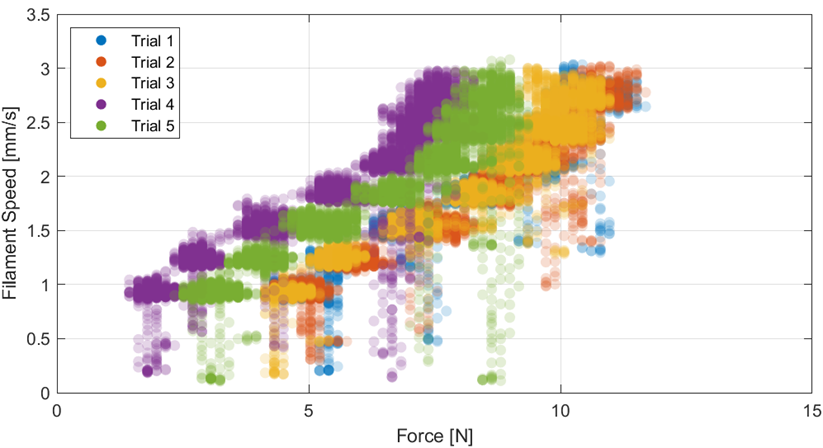
\includegraphics[width=\linewidth, keepaspectratio]{PLA245}
	\caption{Alpha plot for 5 trials of PLA printed at 245°C.} \label{fig:PLA245}
\end{figure}

\begin{table}[!htbp] 
	\renewcommand{\arraystretch}{1.5}
	\centering
	\caption{Average print temperature for PLA 245°C trials.}
	\newcolumntype{C}{ >{\centering\arraybackslash} m{0.25\linewidth} }
	\newcolumntype{M}{ >{\centering\arraybackslash} m{0.15\linewidth} }
	\begin{tabular}{M C} 
		\toprule
		\textbf{Trial} & \textbf{Average Print Temperature $[^\circ C]$}\\
		\midrule
		1 & 241.38\\
		2 & 231.81\\
		3 & 241.23\\
		4 & 251.59\\
		5 & 241.21\\
		\bottomrule
	\end{tabular}
	\label{tab:data_ex_temp_2}
\end{table}

An important observation that can be derived from these experiments is that the data does not fully agree with the Melt Filled Nozzle model proposed by Bellini, Güçeri and Bertoldi \cite{Bellini2004}, nor the Melt Film Model with shear thinning behavior, as modified by Colón et al. \cite{ColonQuintana2020}. Unfortunately, the physical limitations of the setup do not allow for experimentations at higher temperatures or printing speeds, as the drive wheel of the printer would slip, or the heater in the printer would not be able to sustain the elevated temperature while printing. Figure \ref{} shows how the data for a representative case of ABS printed at 230°C compares to the predictions of the Melt Filled Nozzle (FNM) and Melt Film (MFM) models \cite{Bellini2004, OsswaldMelting18, ColonQuintana2020}. ABS printed at 230°C was chosen for this comparison as it proved to be the most consistent condition in all replications of the experiment. The Melt Film model estimations were calculated using two different melting temperatures ($T_m$): the glass transition temperature of the polymer ($T_g$) and $T_g+40K$, as recommended by Colón et al. during his calculations \cite{ColonQuintana2020}. 

\begin{figure}[!htbp]
	\center
	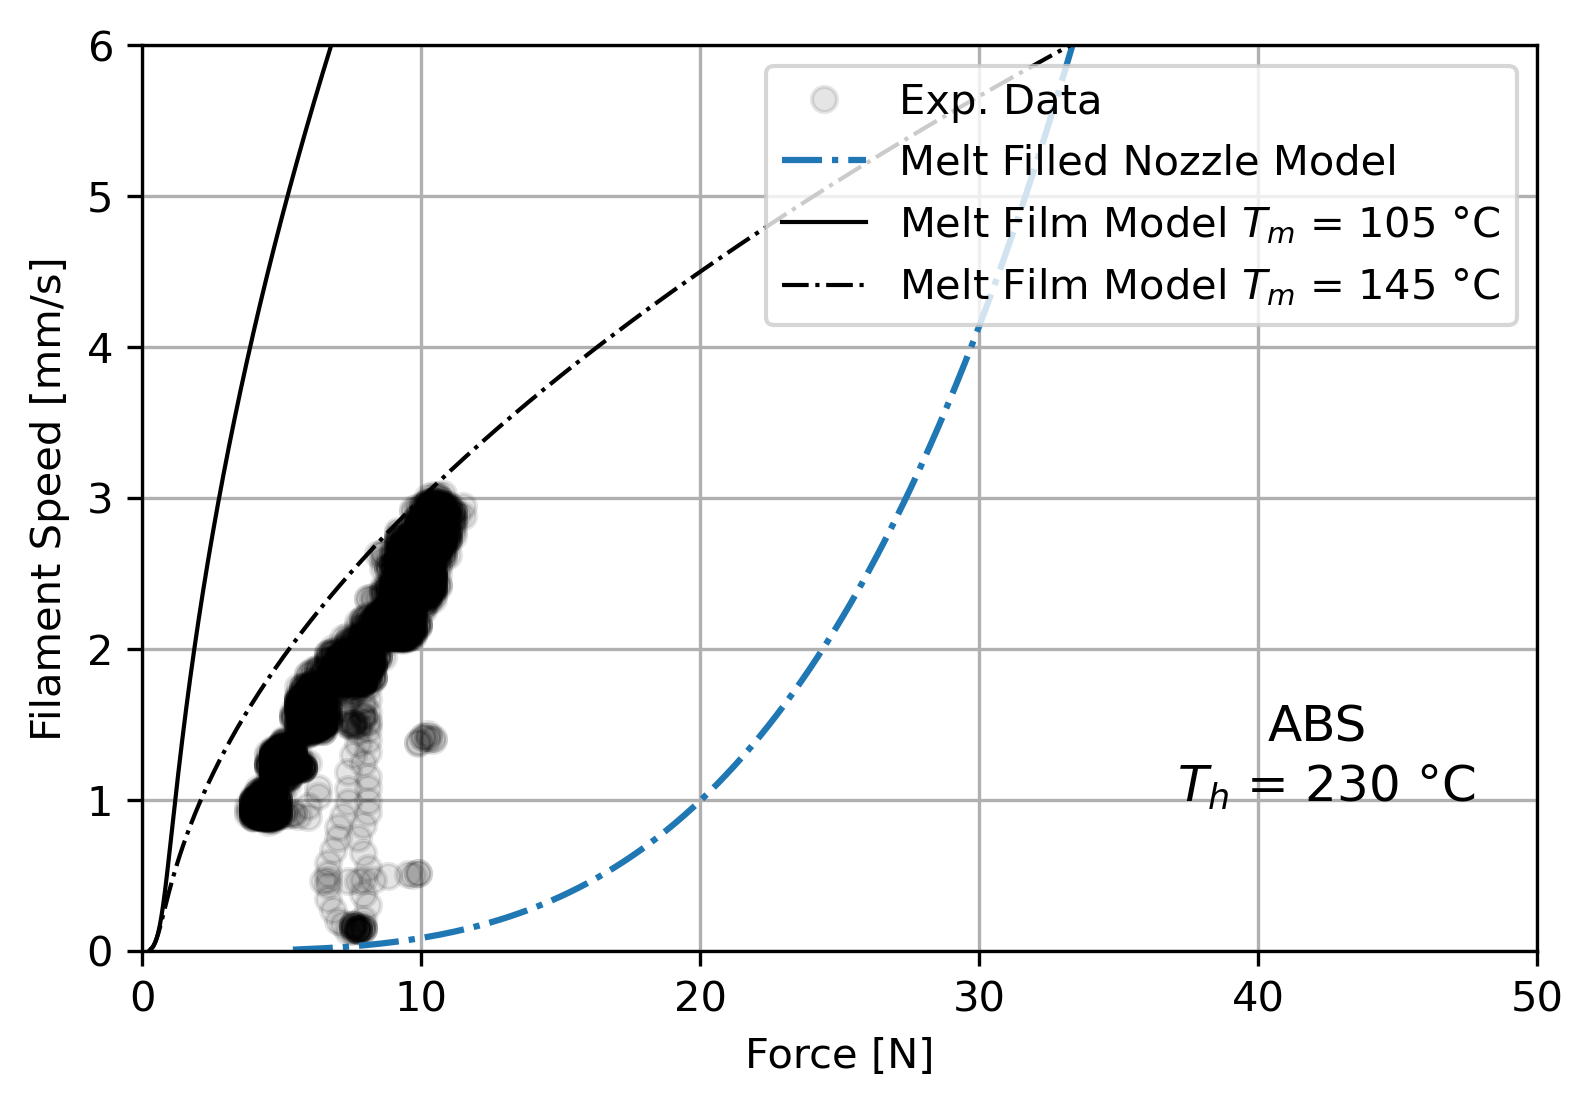
\includegraphics[width=\linewidth, keepaspectratio]{meltcomp}
	\caption{Comparison of experimental data for ABS printed at 230°C with predictions stemming from various ME melting models.} \label{fig:meltmcomp}
\end{figure}

% Nomenclature introduced in this chapter:
\nomenclature[A]{ME}{Material Extrusion}% 
\nomenclature[A]{FNM}{Melt Filled Nozzle Model}%
\nomenclature[A]{MFM}{Melt Film Model}%

\end{document}